\documentclass[conference]{IEEEtran}
\makeatletter
\newcommand{\rmnum}[1]{\romannumeral #1}
\newcommand{\Rmnum}[1]{\expandafter\@slowromancap\romannumeral #1@}
\makeatother

\usepackage{epsfig}
\usepackage{amsopn}
\usepackage{subfigure}
\usepackage{cite}
\ifCLASSINFOpdf

\else
\fi
\usepackage[cmex10]{amsmath}

\interdisplaylinepenalty = 2500

\usepackage{algorithmic}
\usepackage{algorithm}
\hyphenation{op-tical net-works semi-conduc-tor}


\begin{document}
\title{Access Strategy in Super WiFi Network Powered by Solar Energy Harvesting, A POMDP Method}

\author{\authorblockN{Tingwu~Wang\authorrefmark{1},
	Chunxiao~Jiang\authorrefmark{1},
	Yan~Chen\authorrefmark{2},
	Yong~Ren\authorrefmark{1}, and
	K. J. Ray~Liu\authorrefmark{2}}
	\small\authorblockA{\authorrefmark{1}
		Department of Electronic Engineering, Tsinghua University, Beijing, 100084, P. R. China\\
          \authorrefmark{2}Department of Electrical and Computer Engineering,
		  University of Maryland, College Park, MD 20742, USA\\
        E-mail: wtw12@mails.tsinghua.edu.cn, \{jchx, reny\}@tsinghua.edu.cn, \{yan, kjrliu\}@umd.edu}}
\maketitle

\begin{abstract}
The recently announced Super Wi-Fi Network proposal is aiming to enable Internet access in a nation-wide area.
As traditional cable-connected power supply system becomes impractical or costly for a wide range wireless network,
new infrastructure deployment for Super Wi-Fi is needed.
The fast developing Energy Harvesting (EH) techniques receive global
concerns for their potential of solving the above power supply problem.
Many studies have been done on traditional access strategy,
but the access strategy in EH wireless network with multiple Base Stations (BS)
remains a field with tremendous research potential.
Different from traditional wireless network,
a Base Station (BS) in EH powered network harvests energy from the ambient environment.
As the energy is limited,
the BS will not broadcast its system state to all the users within its range,
which leads to incomplete knowledge of the system for the users.
Thus the access strategy has to be carefully chosen.
In this paper, we propose a practical and efficient framework for multiple BSs access strategy
in an EH powered Super Wi-Fi network.
In our work, we consider the access strategy from the a user's perspective,
who exploits downlink transmission opportunities from BS.
To formulate the problem,
we used Partially Observable Markov Decision Process (POMDP) to model the
real world uncertainty.
Simulation results show that our methods are efficacious and significantly outperforms
the traditional widely used CSMA method.
\end{abstract}
\IEEEpeerreviewmaketitle
\section{Introduction}
% ------------------------------------------------------------------------------------------- %
% background
In order to expand the coverage area of wireless network,
many algorithms and implementations have been revised.
And recently, the Federal Communications Commission published the Super Wi-Fi proposal,
aiming to make use of lower-frequency white spaces between television channel frequencies
and create a nationwide wireless network.
However, the ambitious task of building a countrywide network comes across many obstacles.
An inevitable problem is how to deploy practical backhaul and energy supply system.
Traditional cable-based systems are excessive, considering the cost of deploying and maintaining the network,
and sometimes impossible as well as dangerous in complex environment.
Despite all the above difficulties, there are solutions and
many successful experimental deployments of Super Wi-Fi are accomplished accordingly.
Wireless backhual has been proven to be effective \cite{30} as a replacement of cable backhaul.
And the fast developing EH technology provides an ideal replacement as the power supply problem,
which could make use of a wide range of ambient energy including piezoelectric, thermal, solar energy, etc.\\
% ------------------------------------------------------------------------------------------- %
% previous work
\indent As the deployment of EH network is just emerging,
new wireless protocols and modification are needed, as some preliminary studies pointed out \cite{27}.
Previously, the access strategy problem has been a core problem in wireless communications,
and many researchers have been doing some brilliant work in the literature.
Markov Decision Process has been widely used in wireless network,
with some challenges and solutions summarized in \cite{23}.
Access process is a typical game process,
and therefore game theory, summarized in \cite{22},
and pricing theory, used in \cite{7}, has been applied respectively.
In \cite{5}, the access strategy towards multiple BSs with negative externality is considered.
More recently, a POMDP MAC layer opportunistic access is proposed by Dr. Zhao in \cite{zhao1}.
A learning based approach to access between packet bursts is studied in \cite{kae1}.
\\
% ------------------------------------------------------------------------------------------- %
% our work
\indent However, all the mentioned existing studies on the access strategy did not consider the
multiple BSs access strategy under energy harvesting, while, as mentioned above,
using EH powered BSs is the best practicable ways of realizing Super Wi-Fi network.
In this work, we propose an access strategy that is exercisable in the fast booming Super Wi-Fi network.
The special characteristics and their adjoint problems in the EH powered network are studied and solved.
As long time transmission is not guaranteed in EH network,
leaving and arriving of users is more frequent.
Instead of using a static system model,
we consider a model where the number of accessing users and the battery are dynamic.
A revised birth and death process and a battery transition formulation based on quasi-static assumption
are combined to describe system state transition.
Besides, unlike most of the models where the strategy of the users on the BSs is neglected,
we consider the case where an user's decision affects system state.
It is more rational than previous models with no affection.
As, for example, in EH powered network, a user could cause energy depletion,
collision and system low efficiency if it performs short-sighted and selfish strategy,
or causing energy waste when it is too conservative.
And as in EH wireless network, the full knowledge of the system is unrealistic,
a POMDP model is used to formulate the problem, where the information of the system is obtained by observations.
% conclusion about our model
To sum up, we propose an algorithm that is able to overcome the shortcomings in previous models.
And although our work focuses on solar energy harvesting,
it is clear that the conclusion and the algorithm could be generalized to any access problems in EH powered network.
\\
% ------------------------------------------------------------------------------------------- %
% organization
\indent The rest of this paper is organized as follow.
We describe the system model In Section \Rmnum{2}.
In Section \Rmnum{3}, the POMDP access strategy is presented.
We show how we formulate the POMDP states to obtain the optimal access strategy. 
And a suboptimal strategy is proposed.
In Section \Rmnum{4}, we evaluate the performance of our proposed approach with several famous traditional algorithms.
In Section \Rmnum{5} we draw the conclusion.
% ------------------------------------------------------------------------------------------- %
% ----------------------------end of introduction-------------------------------------------- %
% ------------------------------------------------------------------------------------------- %
\section{System Model}
As shown in Fig. 1, in an EH network, there are multiple BSs.
Each BS is supplied by EH devices and connected to the server by wireless backhaul.\\\indent
In each time slot, the BS harvests a certain quantity of solar energy, 
denoted as \(E_H\), and stores it into its battery.
At the same time, to serve the users connected to the BS, energy \(E_T\) is consumed for transmission.
We denote the battery quantity of the BS as \(Q_B\),
which could be any values from \(0\) to the battery volume \(B_M\).
In the network, there are different types of users.
And in every times slot, the BSs could serve multiple users,
the number of which is denoted as \(S_U = i,\, i = \,0,\,1,\,\ldots,\,N_U-1\).
\(N_U\) is the maximum number of users the BS could serve simultaneously due to limited spectrum and coding ability.
Note that different BSs in the network could have different battery volume \(B_M\) and maximum serving users \(N_U\).\\\indent
At the start of each time slot,
users with new service demand could decide either to access or sense one of the BSs within its range.
We denote the action as \(\Phi = \Phi_{a}^i\) for accessing the \(i^{th}\) BS,
and \(\Phi = \Phi_{s}^i\) for sensing.
In the case of sensing,
the BS will respond to the user by sending its next-time-slot system state
in a short message which requires negligible energy consumption.
In the case of accessing, the user sends a request to the chosen BS.
When the request is achievable, BS will activate user's transmission immediately.
When the request is unavailable, the BS will decline the request and
inform the user its next-time-slot system state, again with a low energy consuming short message.
In the above process, the short message could
be used as observation to update the belief of the system state by the user.
Clearly, the action has to be careful chosen.
On the one hand, the user wants to maximize its utility by making enough many access attempts.
On the other hand, senseing is necessary,
as the lack of information will result in useless attempts, causing energy waste and access failures.\\
\indent
From the BSs' perspective, certain protections are needed,
as users could malicious keep accessing one BS and use up all the energy.
To focus our work on formulation from the user perspective and
not to be distracted by protection details,
a simple protection is used in our work.
If a BS is currently not serving any users and the battery is low,
the BS will reserve the last quantity of energy that could serve a user
for one time slot and forbid new users from using it.\\\indent
In our work, we consider a rational user who could observe multiple BSs and
chooses an action in every time slot to maximize its number of successful access.
The number of the observed BSs by the user is denoted as \(N_A\).
\begin{figure}\label{fig1}
\centering
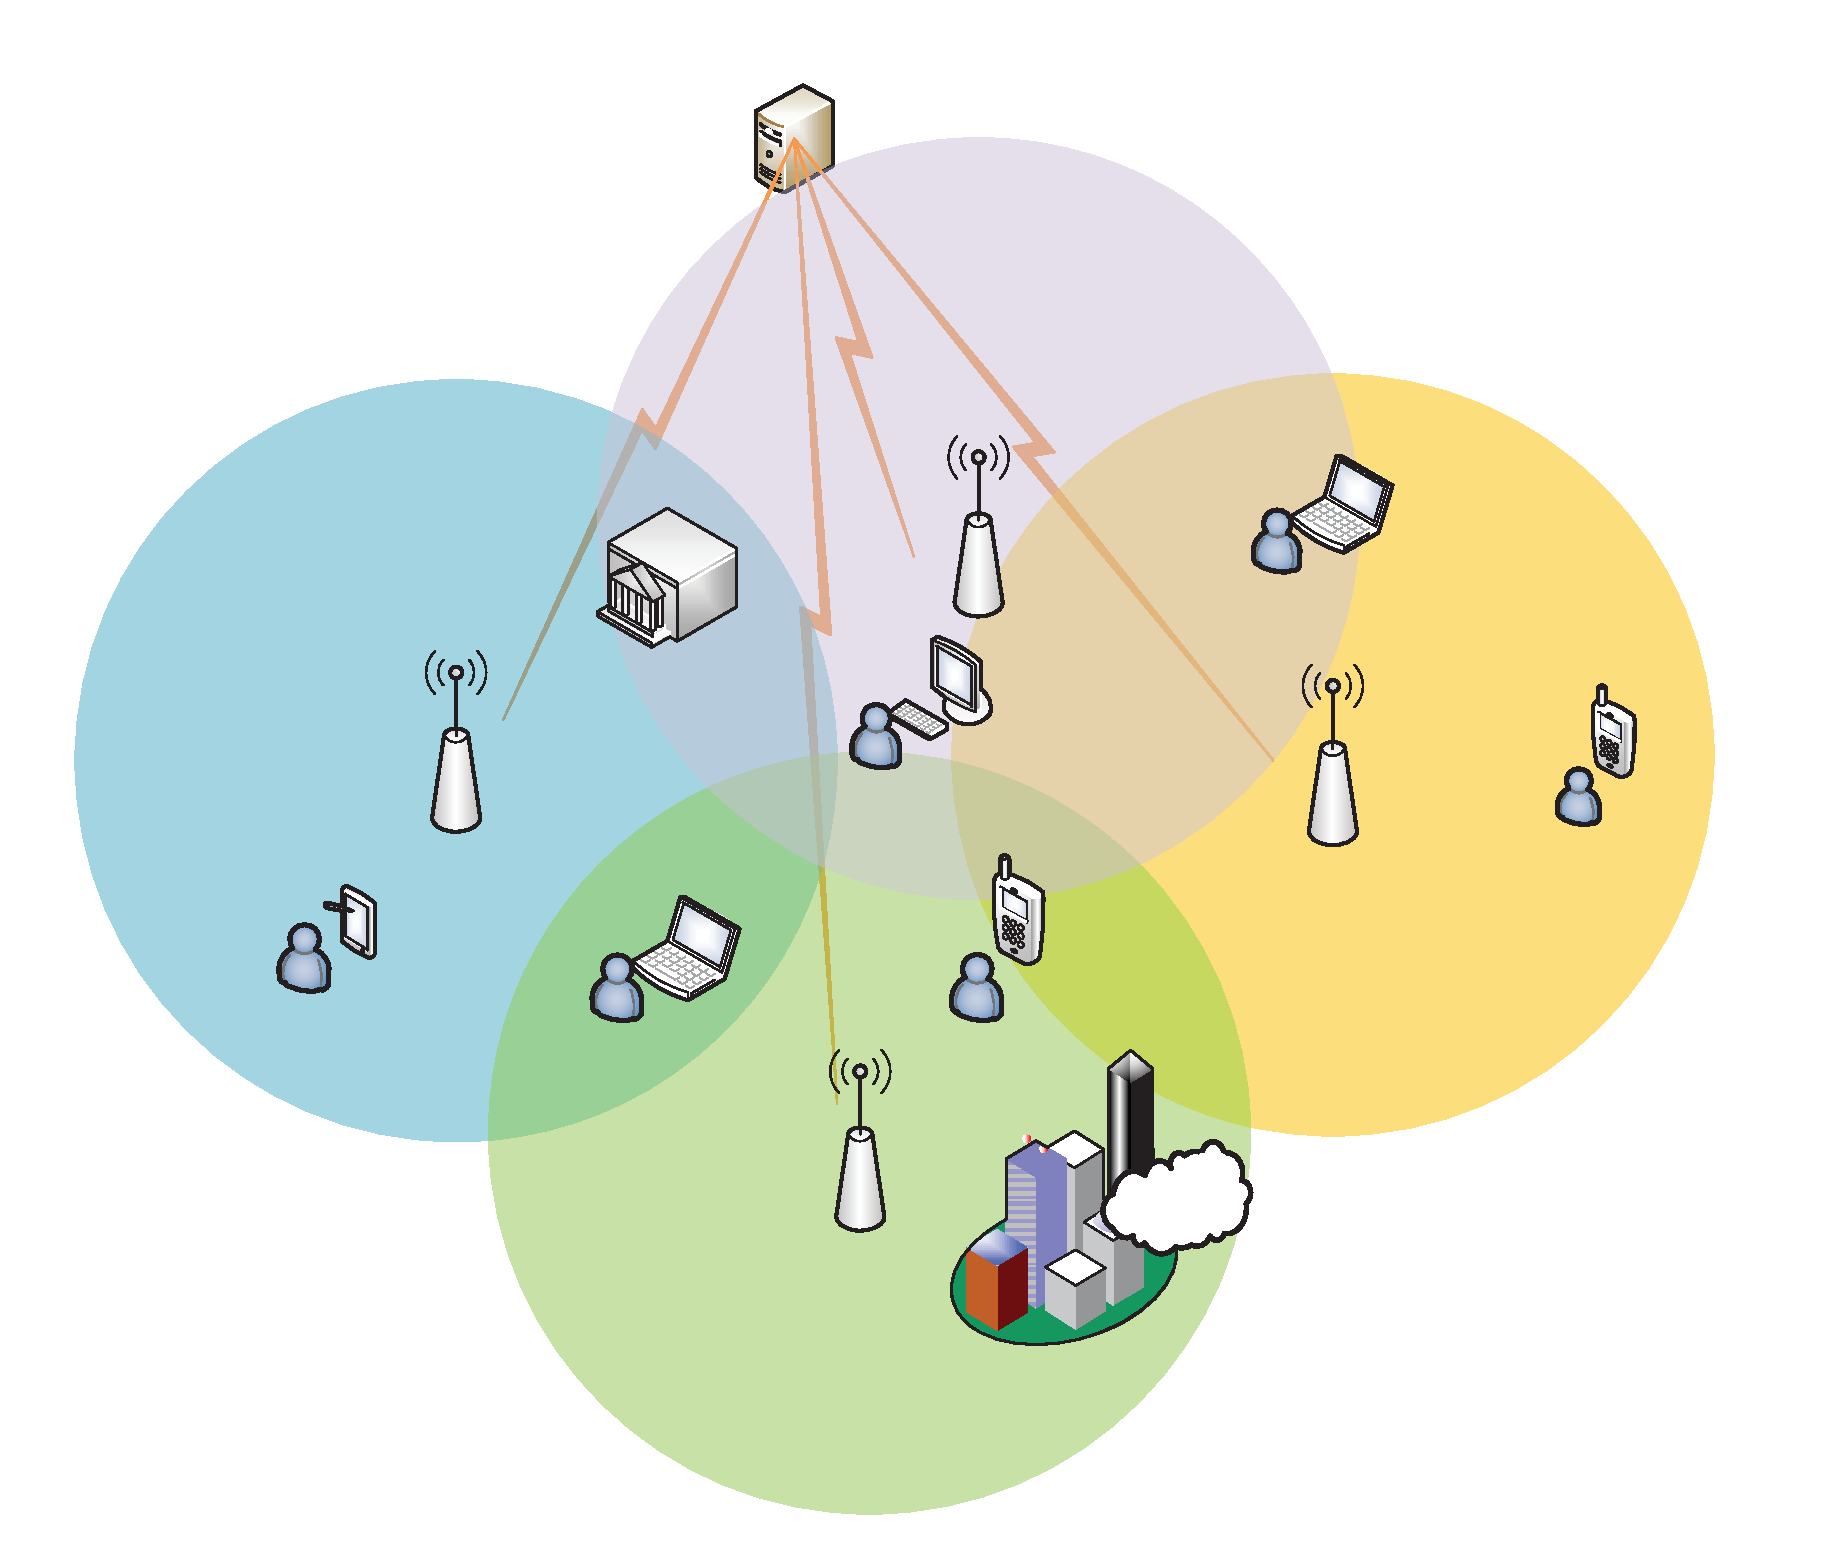
\includegraphics[width=8.5cm]{Fig1.eps}
\caption{A schematic map of Super Wi-Fi system.}
\end{figure}
\section{POMDP Access Strategy}
As POMDP could solve decision making problems of different decision horizon lengths under uncertainty,
it perfectly depicts the above EH Super Wi-Fi model.
In order to formulate the problem, two key components in the system model, user number and battery, are carefully considered.
%Before formulating our proposed algorithm by POMDP,
%it is important to define our system states and state transition.
\subsection{User Model}
%During each time slot, a certain quantity of energy,
%denoted as \(E_H\) is harvested from external environment.
%And at the same time, a quantity of energy \(E_T\) is consumed for transmitting wireless signal.
% ------------------------------%%%%%%%%%%%%%%%%%%%%%%
Like in traditional wireless network, the users arrive and leave the BS with certain probability \cite{5}.
Between adjacent time slots, new users may arrive and
old users may actively leave or be forced to leave when battery is insufficient.
A revised birth and death process that considers forced leaving are proposed as follow,
\begin{align}\label{formula1}
&\zeta\left(S_U'| S_U, Q_B, \Phi\right) = \nonumber\\
&\begin{cases}
	\lambda, &\mbox{if $Q_B$ is enough and $S_U' = S_U + 1$,}\\
	\mu S_U, &\mbox{if $Q_B$ is enough and $S_U' = S_U - 1$,}\\
	I_0\left(S_U'\right), &\mbox{if $Q_B$ is insufficient,}\\
	0, &\mbox{otherwise.}\\
\end{cases}
\end{align}
In the above equation, \(\lambda\) is the arriving rate and
the \(\mu' = \mu S_U\) is the leaving rate of users.
The forced leaving is formulated by the indicator function \(I_0\left(S_U'\right)\),
which indicates that \(S_U'\) next time slot is sure to be \(0\).
Energy depletion happens when \(Q_B- E_T \leq 0\).
\subsection{Battery Formulation}
The harvested energy \(E_T\) is determined by the environmental parameters.
Gaussian models have been proved effective in predicting solar intensity \cite{gaussian,data}.
The harvest model assumes that the solar intensity in a long time period are Gaussian distributed.
And the solar intensity during one single time slot, the length of it denoted as \(T_L\), remains unchanged.
Thus the solar intensity \(W_e\) could be formulated as
Gaussian distributed \(\mathcal{N}\left(x;\mu_S,\sigma_S\right)\)
with average intensity \(\mu_S\) and variance \(\sigma_S^2\).
In current devices,
the harvesting power per reference solar intensity is
\(E_H = W_eJ_{op}V_{op}\Omega_ST_L\eta\), where the \(J_{op}\) and \(V_{op}\) is the optimal operating point,
the \(\Omega_S\) is the number of solar cells and the \(\eta\) is the efficiency \cite{physic}.\\
\indent The transmitting power is set by BSs to provide enough SINR for the receiving users.
Current power adjustment algorithms that use feedback are not valid,
as the system state are fast changing between time slots.
Therefore here a static power management is implemented,
where the BS sacrifices some energy to insure a successful transmission every time slot.
%choose the transmitting power by considering the worst case,
%which includes for example assuming that users are all at the edge of its cell.
The power consumption in a BS is determined by the number of accessing users,
which is denoted as \(E_T = \Upsilon_T(S_U, Q_B, \Phi)\).
As wide range telecommunication has negligible between-user interference,
we assume the transmission power is proportional to the number of serving users, i.e.,
\(\Upsilon_T(S_U, Q_B, \Phi) = P_T(S_U + \Theta(S_U,Q_B,\Phi_a))\), where \(P_T\) is the transmission power for single user.
\(\Theta(S_U,Q_B,\Phi_a)\) is \(1\) if the rational user could successfully access, otherwise it is \(0\).
Correspondingly, we assume the battery volume \(B_M = \rho P_TT_L\), where \(\rho\) is an integer.
Note that for the nonlinear transmission power function,
our method could still work by setting different battery levels in the below sections.
%Naturally, a successfully accessed rational user is equivalent to an extra ordinary user to the BS, i.e.,
%for BS \(i\), the transmitting power satisfies
%\(\Upsilon_T(S_U, Q_B, \Phi = \Phi_{a}^{i}) = \Upsilon_T(S_U + 1, Q_B, \Phi \ne \Phi_{a}^i)\).
When the required battery is more than the BS's remaining battery,
the BS will provide a best effort service.
Users with the higher priority are served.
In our case, the rational user has the lowest priority.
Given the \(E_H,\,E_T\), the battery in the next time slot could be calculated as,
\begin{equation}
	Q_B' = \mbox{min}\{Q_B + E_H - E_T, B_M\}.
\end{equation}
\indent In EH powered BSs, the battery is a continuous value.
But in a POMDP, the states have to be discrete.
Intuitively, we could use more battery states to approximate continuous value,
but this brings much increase in the complexity of the algorithm.
Luckily, a certain number of discrete levels could provide enough information during the decision making.
We could set battery levels according to the possible energy consumption in each time slot \(T_L\Upsilon_T(S_U,Q_B,\Phi)\).
In the case of linear power function, the levels are set as \(S_B = \lfloor Q_B / \left(P_TT_L\right) \rfloor\).
And the number of battery states is \(N_B = B_M / \left(P_TT_L\right) +1 = \rho + 1\).
Thus, by knowing the battery states,
the user would know whether the battery is sufficient for transmission.\\
\indent
The prediction of future battery states are base on transition probability between battery states.
In order to calculate the transition probability,
we assume the fluctuate of discrete battery state is quasi-static.
i.e., the residue energy \(Q_B - S_BP_TT_L\) is uniformly distributed between \(\left[0,\,P_TT_L\right)\).
Clearly errors are brought by this assumption,
but the quasi-static assumption is proven to be effective after a large number of time slots \cite{data}.
We denote the change of battery state between time slot as \(\Delta_B = S_{B}' - S_B\).
Event \(\xi_j\) represents that the real battery quantity change \(E_H - E_T\)
is equivalent to more than \(j\) but less than \(j+1\) battery state change, namely
\(\xi_j := \{j\leq \frac{E_H - E_T}{P_TT_L} \le j+1\}\).
Then the probability that the battery state will change by \(\Delta_B\)
given \(E_H\) and user action could be computed as follow,
\begin{align}&\mbox{Pr}\left(\Delta_B = i |\Phi, E_H, \xi_j \right)\nonumber\\
=&\begin{cases} \frac{\left(E_H - E_T\right)}{P_TT_L} -j, &\mbox{$i = j + 1$},\\
\left(j+1\right) -\frac{\left(E_H - E_T\right)} {P_TT_L}, &\mbox{$i = j$},\\
0, &\mbox{otherwise.}\\
\end{cases}
\end{align}
In the equation, as mentioned in previous section, \(E_T = \Upsilon_T(S_U, Q_B, \Phi)\).
When \(E_H - E_T \le 0\), the probability could be calculated the same way.
The battery transition is then,
\begin{equation}\label{battery}
\begin{aligned}
	&\mbox{Pr}\left(\Delta_B = i |\Phi\right) = \\
	&\int\nolimits_{i\epsilon_T + E_T}^{\left(i+1\right)\epsilon_T+ E_T}
	\mbox{Pr}\left(\Delta_B = i |\Phi, E_H, \xi_i\right) \mathcal{N}\left(E_H;\bar{\mu_S},\bar{\sigma_S}\right) dE_H+\\
	& \int_{\left(i-1\right)\epsilon_T+ E_T}^{i\epsilon_T + E_T}
	\mbox{Pr}\left(\Delta_B = i |\Phi, E_H, \xi_{i-1}\right) \mathcal{N}\left(E_H;\bar{\mu_S},\bar{\sigma_S}\right) dE_H.\\
\end{aligned}
\end{equation}
In the equation, \(\epsilon_T = P_TT_L\) and \(\bar{\mu_S},\,\bar{\sigma_S}\)
are scaled from \(\mu_S,\,\sigma_S\) after the multiplication with harvesting device coefficients.
\subsection{System Transition Probability}
%When the user transition probability and battery transition probability is computable,
%we could focus on the formulation of POMDP.
The POMDP state is the overall system state, which combines all the BSs' system state.
To make the following math more readable and flexible,
the system state \(S\) and \(S_D = \{S_B^1,\,S_U^1,\,\ldots,\,S_B^{N_A},\,S_U^{N_A}\}\)
are equivalent and used simultaneously.
We have \(S = 1,\,2,\, \ldots\,N_S\), where \(N_S = \left(N_BN_U\right)^{N_A}\).
We first calculate the transition probability for a single BS.
From conditionally independence we have
\begin{equation}
\begin{aligned}
	\mbox{P}\left(S_U',S_B'|S_U,S_B,\Phi\right) =
	\zeta\left(S_U'|S_U, S_B, \Phi\right) \delta\left(S_B'|S_U, S_B, \Phi\right).\\
\end{aligned}
\end{equation}
The \(\zeta\left(S_U'|S_U, S_B, \Phi\right)\) is given in equation \eqref{formula1}.
And the battery transition is calculated based on the equation \eqref{battery},
\begin{align}
	&\delta\left(S_B'|S_U, S_B, \Phi\right)\nonumber\\
	= &
	\begin{cases}
		\mbox{Pr}\left(\Delta_B = S_B' - S_B|\Phi \right), &\mbox{if $S_B' \le N_B - 1$,}\\
		\sum_{\Delta_B = S_B' - S_B}^{\Delta_B = \Delta_B^{Max}}\mbox{Pr}\left(\Delta_B|\Phi\right),
		&\mbox{if $S_B' = N_B - 1$.}\\
\end{cases}
\end{align}
When the battery is fully charged, \(S_B'=N_B - 1\), all the extra harvested battery is abandoned.
Note that we truncate the probability for \(\Delta_B >\Delta_B^{Max}\) as they are as small as zero by \(4\) decimals.
Thus the POMDP state transition is computed as,
\begin{align}\label{transition}
	T\left(S'|S,\Phi\right) = \prod_{i = 1}^{i = N_A}\mbox{P}\left(S_B^{i,'}, S_U^{i,'}|S_U^i, S_B^i, \Phi\right).
\end{align}
\subsection{Observation Function and POMDP Iteration Algorithm}
In POMDP formulation, the user only has the partial knowledge of the system.
As mentioned above, the user could get the target BS's next-time-slot system state
\(S_B^O\) and \(S_U^O\) at the end of each time slot.
We use observation \(O\) to represent \(S_B^O,\,S_U^O\).
The observation probability function given the system state in the next time slot is
\begin{align}
	Z\left(O|S',\Phi\right) = \mbox{Pr}\left(O\Big|S_U^{t,'}, S_B^{t,'}\right) =
	I_{S_U^{t,'},S_B^{t,'}}\left(S_U^O, S_B^O\right).
\end{align}
\(S_B^{t,'}\) and \(S_U^{t,'}\) are the system state of the target BS next time slot.
The indicator function is \(1\) when \(S_U^{t,'} = S_U^O,\,S_B^{t,'}=S_B^O\) or \(0\) otherwise.\\\indent
The reward is define as \(R = 1\) if the access succeeds, else \(R= 0\).
Then the value function of a single state is,
\begin{equation}
\begin{aligned}
	V_t^\Phi\left(S\right) = R\left(S,\Phi\right) +\gamma\sum\limits_{S'}T\left(S'|S,\Phi\right)V_{t-1}^\pi\left(S'\right),
\end{aligned}
\end{equation}
where \(\pi\) denotes the optimal action in that state.
As no full knowledge is held for the user, we use a belief vector to denote the user's system state belief
\(\beta = \lbrack \beta\left(S = 1\right),\,\beta\left(S = 2\right),\,\ldots,\,\beta\left(S = N_S\right)\rbrack\).	
Then the particular value function with a certain belief \(\beta\) is given as
\begin{equation}
\begin{aligned}
	V_t^\Phi\left(\beta\right) = & \sum\limits_{S}R\left(S,\Phi\right)\beta\left(S\right) +\\
	&	\gamma\sum\limits_{S}\sum\limits_{S'}\beta\left(S\right)T\left(S'|S,\Phi\right)V_{t-1}^\pi\left(S'\right).
\end{aligned}
\end{equation}
For simplicity, if we already know all the value function of at the time \(t-1\) during iterations,
an alpha value vector \(\alpha_t^\Phi = \lbrack \alpha_t^\Phi\left(S = 1\right),\,
\alpha_t^\Phi\left(S = 2\right),\,\ldots,\,\alpha_t^\Phi\left(S = N_S\right)\rbrack\)
could be used to simplify the value function as
\(V_t^\Phi\left(\beta\right) = \sum\beta\left(S\right)\alpha_t^\Phi\left(S\right)\).
Thus the optimal action is given as,
\begin{equation}
\begin{aligned}
	\pi\left(\beta\right) =
	\arg\underset{\alpha_t^\Phi}{\max}\sum\limits_{S}\beta\left(S\right)\alpha_t^\Phi.\\
\end{aligned}
\end{equation}
The corresponding value function \(V_t^\Phi\left(\beta\right)\) could be calculated using action \(\pi\left(\beta\right)\).
However, the corresponding optimal policy is not as easy as it seems to be, as the \(\beta\) has a continuous value,
and even for the same \(\Phi\) and \(t\), there are still multiple possible \(\alpha\) vectors during iterations.
But fortunately, the \(V_t\) could be regarded as the function value of \(\beta\) in a hyper coordinate system,
the axes of which are the components of \(\beta\).
As each set of \(\alpha_t\) vector could be regarded as a set of parameters of a hyper linear function,
there is a dominated hyperplane structure in the model.
The continuous belief space is divided by several \(\alpha\)-vector-dominated hyperplanes into several partitions.
The partitions of belief space in time \(t\) could be calculated given all the dominating \(\alpha_{t-1}\).
The details of algorithm for solving the partitions could be find in a well written tutorial \cite{pomdptool}.\\
\indent
After obtaining the optimal action, the user could act accordingly,
and update its belief vector after receiving the observation by using the below formula.
\begin{align}
	\beta'\left(S'|\Phi, O\right) = \frac{\sum_{O}Z\left(O|S',\Phi\right)\sum_{S}
	T\left(S'|S,\Phi\right)\beta\left(S\right)}
	{\sum_{S'}\sum_{O}Z\left(O|S',\Phi\right)\sum_{S}T\left(S'|S,\Phi\right)\beta\left(S\right)}.
\end{align}
\begin{figure}
\centering
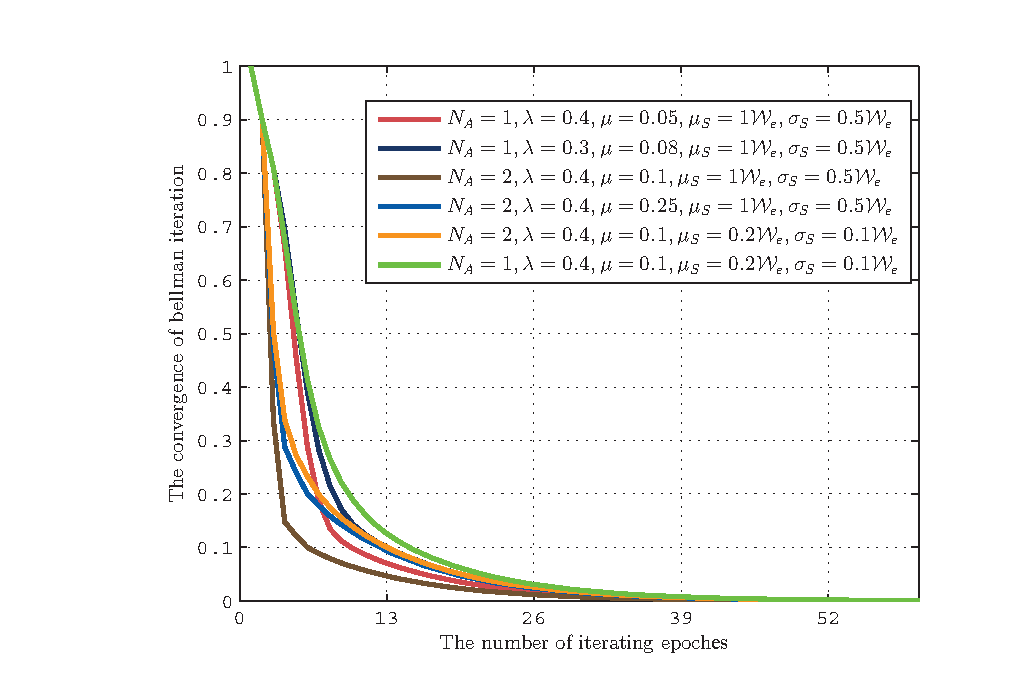
\includegraphics[width=8.5cm]{2_fig3.eps}
\caption{Illustration of the convergence of the POMDP iteration algorithm}
\end{figure}
\subsection{Suboptimal Access Policy}
The optimal POMDP solution could be calculated off-line within seconds when the number of states is small.
However, the use of POMDP method is limited when \(N_A\) is massive,
and when the environment parameters, like solar coefficients \(\mu_S\), \(\sigma\),
the birth rate \(\lambda\) and death rate \(\mu\) of users, change quickly.\\
The POMDP formulation will maximize success access ratio \(\eta_A = N_S/N_T\),
where \(N_S\) is number of success access and \(N_T\) is the number of the time slots.
We propose a dual perspective of solving the problem by focusing on the harvested energy.
We name it Energy Based (EB) Method.
The problem is reformulated as,
\begin{equation}
\begin{aligned}
	\underset{\Phi_t,t=0,\,\ldots,\,N_T-1}{\max}\sum\nolimits_{t=1}^{N_T}
	\mbox{E}\big[\,\mbox{H}\left(\beta^t, \Phi_t\right)\big],\\
\end{aligned}
\end{equation}
where the expectation function E[\(\cdot\)] considers the probability of receiving different observations 
and thus having different belief vector \(\beta^t\).
In the equation,
\begin{equation}
\begin{aligned}
	\mbox{H}\left(\beta^t, \Phi_T\right) = \sum\beta^t\left(S\right)\sum_{i=1}^{N_A}
	\mbox{min}\left(E_H^i,\,E_T^i+B_M-Q_B^i\right)
\end{aligned}
\end{equation}
is the overall harvesting energy in all the BSs combined.
Now a suboptimal could be proposed by maximizing the system's next-time-slot harvested energy.
\begin{equation}
\begin{aligned}
	\Phi\left(\beta^t\right) = \arg{\max}\,\,\mbox{E}\big\lbrack\,\mbox{H}(\beta^{t+1}, \Phi_t)\big\rbrack,\\
\end{aligned}
\end{equation}
When sense is the best action, the user will choose to sense the BS that is not sensed for the longest time.
Due to the limited space, some key rationality of the EB method is summarized.
First of all, when the solar intensity is strong,
we could assume few users will be forced to leave and thus the consumed energy by them are stable.
As the transmission power is proportional to number of users,
we could deduce that the more energy the system harvests,
the more utility the rational user could achieve.
Besides, the EB method is an unselfish method, which would sacrifice some reward,
but tends to protect overall utility.
And EB method could use learning algorithm to adjust to quick environmental changes.
\section{Simulation Results}
\begin{figure}[t]
\centering
\subfigure[The utility ratio with arrival rate in single BS]{
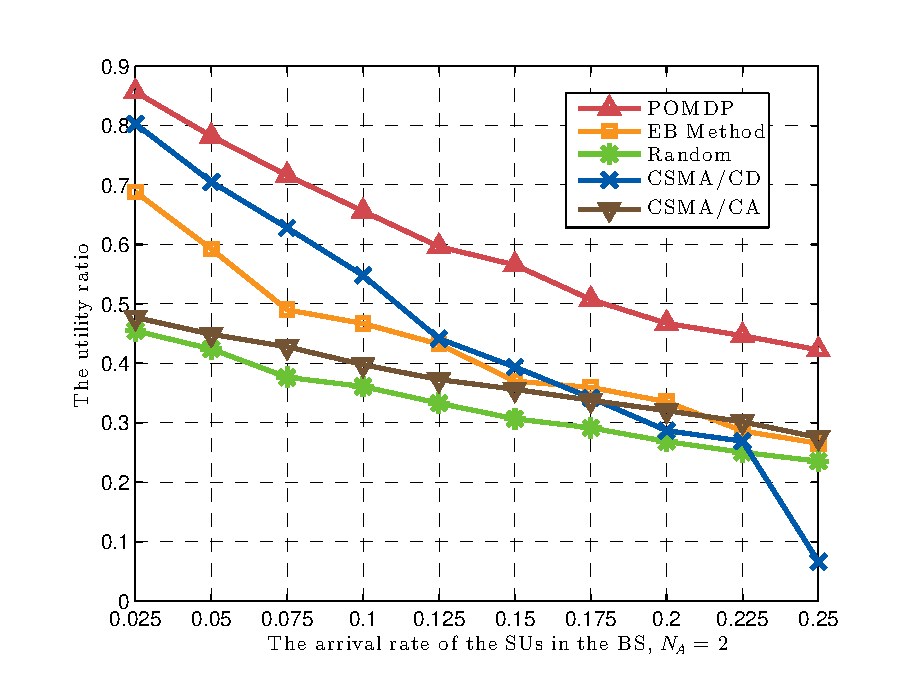
\includegraphics[width=0.5\textwidth,height=6.7cm]{3_fig1_1.eps}}
\subfigure[The utility ratio with solar intensity in single BS]{
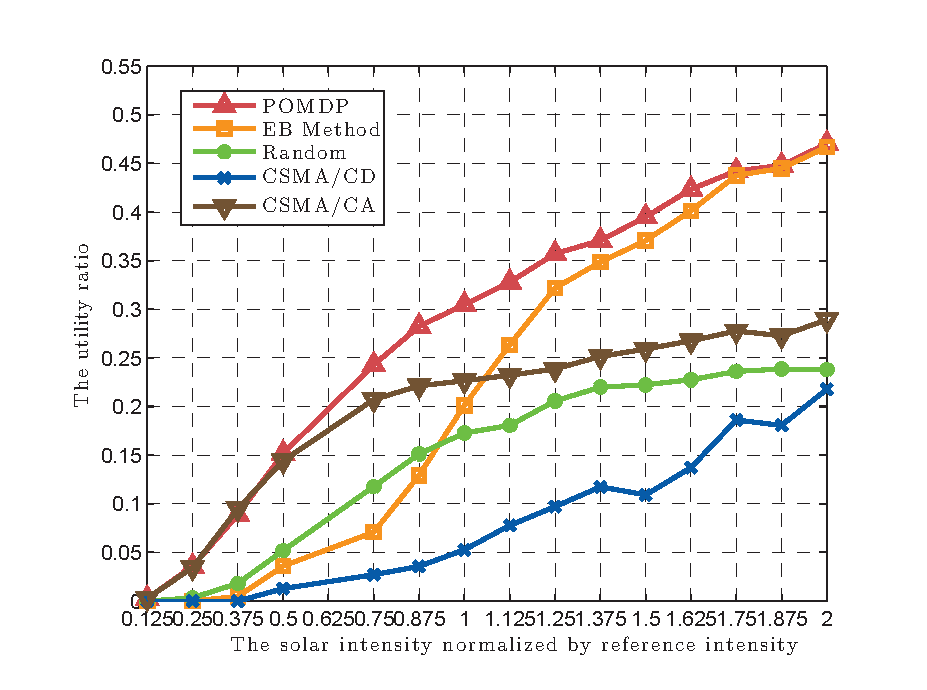
\includegraphics[width=0.5\textwidth,height=6.7cm]{3_fig2_2.eps}}
\caption{Single BS with \(S_U = 0,\,1,\,2,\,3,\, N_B = 8\)}
\end{figure}
\begin{figure}[t]
\centering
\subfigure[The utility ratio with arrival rate in two BS]{
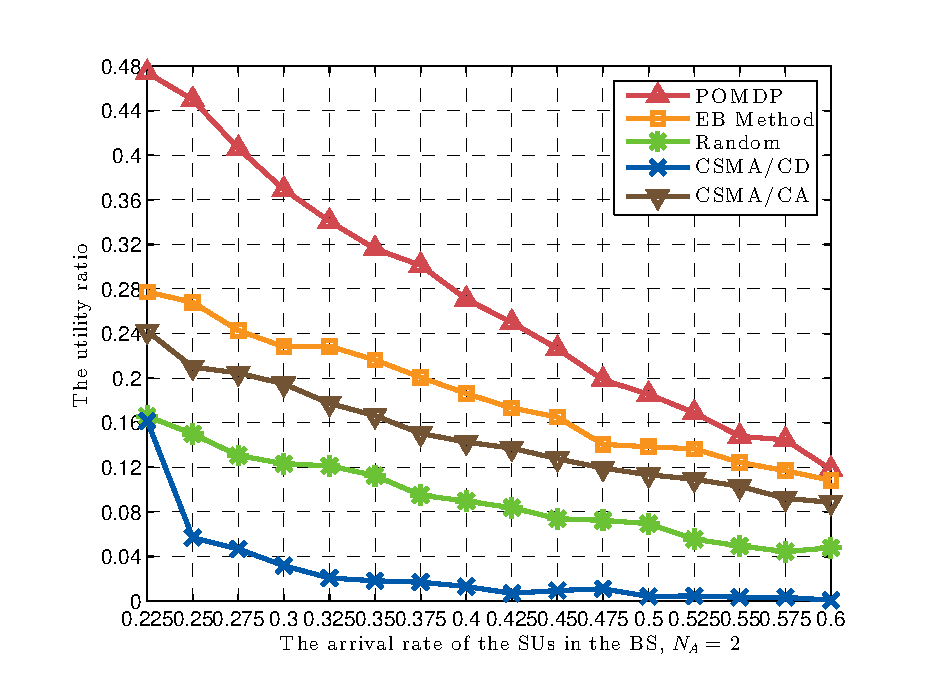
\includegraphics[width=0.5\textwidth,height=6.7cm]{3_fig2_1.eps}}
\subfigure[The utility ratio with solar intensity in two BS]{
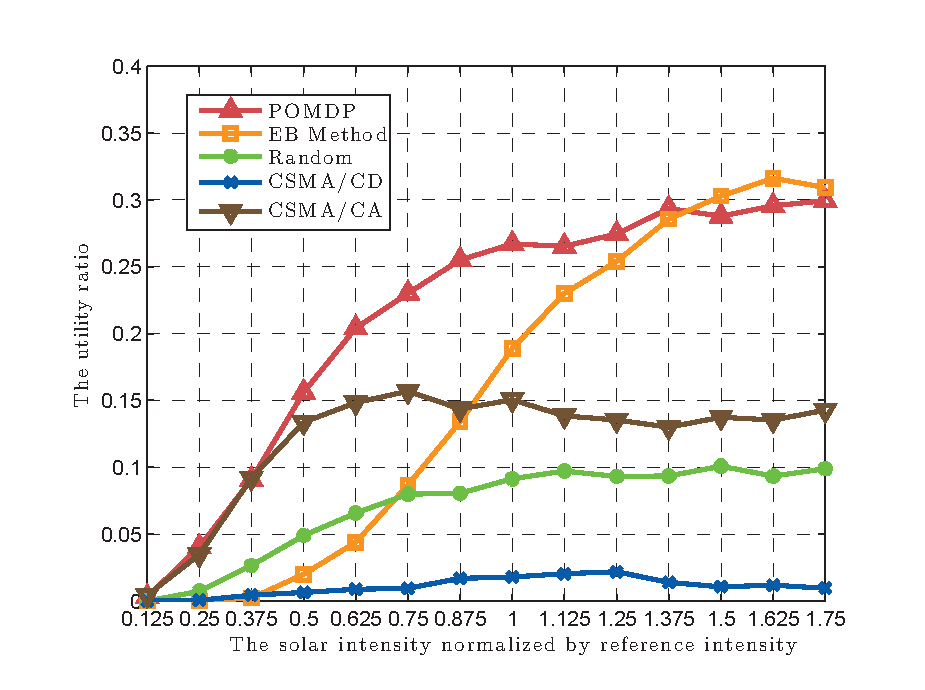
\includegraphics[width=0.5\textwidth,height=6.7cm]{3_fig1_2.eps}}
\caption{Two BS with \(U_N = 0,\,1,\, N_B = 3\)}
\end{figure}
In this section, the convergence and effectiveness of the algorithm is illustrated.
In Fig. 2, the convergence of the POMDP iteration algorithm is shown, where the discount factor is \(\gamma = 0.9\).
A bellman stoping criteria is used to determine the stop of iteration.
In the figure, the \(\alpha\) vector error shows the convergence of the iteration algorithm.
The POMDP simulation tool is provided by \cite{pomdptool}.
As is clear in the fig, the algorithm converges exponentially.\\
% ------------------------------------------%
\indent The effectiveness of the algorithms is validated by comparing the \(\eta_A\)
under the overall time slots \(N_T = 10000\).
In the simulation, parameters are used as follow.
The reference benchmark solar intensity is given as \(\mathcal{W}_e = 1\mbox{kW}/m^2\),
which is the average intensity on the surface of Earth \cite{electric}.
We use the date from work \cite{circuit}, where the optimal power per benchmark solar intensity \(\mathcal{W}_e\)
is \(P_H = J_{op}V_{op} = 1.32\mbox{mW}/\mathcal{W}_e\), with a efficiency \(\eta = 75 \%\).
And there are \(\Omega_S = 40\) cells in one harvesting device.
The time slot length is \(T_L = 200\mbox{ms}\).
Transmission power for serving one user is \(P_T = 40\mbox{mW}\).\\
\indent In order to show the efficiency, several algorithms are implemented as comparisons.
CSMA/CA and CSMA/CD are used.
Slightly different from the standard CSMA, the users sense the BSs instead of the carrier.
And the algorithm tries to avoid all kinds of access failures, not just collision.
The CD method will stop requests when detecting a failure. A exponential back-off algorithm is used.
After \(c\) failures, a random number of sleeping time slot between \(0\) and \(2^c - 1\) is chosen.
The CA method will only access after the user senses the BS in the last time slot
and knows that a successful service is available.
In random access algorithm, the user simply chooses action with equal probability.\\
\indent In Fig. 3, we consider single BS with possible number of users from \(0\) to \(3\), \(N_B = 8\),
and the leaving rate \(\mu = 0.05\).
In Fig. 3 (a), the \(\mu_S = 1\) and \(\sigma_S = 0.5\). In Fig. 3 (b), the arrival rate \(\lambda = 0.4\).
As shown in the figure, the performance of proposed POMDP is significantly higher,
with the EM method's overall performance following at the second place,
which validates the efficiency of our algorithms.
From (a), the CSMA/CD has a good performance when the system is not busy,
but the performance deteriorates quickly with the increasing arrival rate of users.
From (b), it is also clear that even when the solar intensity is strong,
the traditional algorithms' ability to increase utility is still largely limited.
Traditional algorithms are not able to make use of the EH information of the system.
It is also worth noting that, as we predicted, when the solar intensity is strong,
the suboptimal EB method will approach the proposed POMDP method.\\
\indent In Fig. 4, multiple BSs are considered, with possible number of user from \(0\) to \(1\),
\(N_B = 3\), and the leaving rate \(\mu = 0.05\).
Besides what is shown in Fig. 3, we also find in Fig. 4
that when the possible serving positions is limited, the crowded system makes the CSMA/CD method almost useless.
In (b), a simple analysis of the CSMA/CD performance could be given.
When the solar intensity is small, the utility of CSMA/CD increases with intensity due to more available sources.
But when the solar intensity is strong, as the more users are staying in the BS,
the user has less chances of being served, and the utility decreases.
Also, in (b), the suboptimal EB method could outperform POMDP method when the intensity is strong,
which is mainly brought by the errors caused in the POMDP formulation, like using the quasi-static assumption.
\section{Conclusion}
In this paper, we proposed a powerful POMDP algorithm to solve the access problem in EH powered network,
which is promising and instructive in building a national range Super Wi-Fi network.
The framework given in this paper is adjustable to EH problems other than the Solar EH one.
To reduce complexity and adjust to environmental changes, a suboptimal EB method is proposed as well.
The affect of solar intensity, user arriving rate, leaving rate and many other features are considered,
proving our work reliable and effective.
Future work of this paper could focus on the prediction of system parameters and multiuser accessing scenario.
\bibliographystyle{IEEEtran}
\bibliography{Ref}
\end{document}
